\documentclass[11pt,a4paper]{article}

\usepackage[margin=0.84in,top=0.81in,bottom=0.81in]{geometry}
\usepackage{amsmath,amssymb,mathtools}
\usepackage{booktabs,array}
\usepackage{graphicx}
\usepackage{xcolor}
\usepackage{xeCJK}
\xeCJKsetup{CJKspace=true}
\usepackage[most]{tcolorbox}
\usepackage{fancyhdr}
\usepackage{titlesec}
\usepackage{hyperref}
\raggedbottom
\emergencystretch=1.5em

\setCJKmainfont[BoldFont={NanumMyeongjoExtraBold}]{Nanum Myeongjo}
\setCJKsansfont{Apple SD Gothic Neo}
\linespread{1.12}
\setlength{\parskip}{0.22em}
\setlength{\parindent}{0pt}
\renewcommand{\figurename}{{\sffamily\bfseries 그림}}
\renewcommand{\tablename}{{\sffamily\bfseries 표}}

\definecolor{navy}{HTML}{0F172A}
\definecolor{royal}{HTML}{1D4ED8}
\definecolor{teal}{HTML}{0D9488}
\definecolor{rose}{HTML}{BE123C}
\definecolor{amber}{HTML}{B45309}
\definecolor{softbg}{HTML}{F8FAFC}
\definecolor{softteal}{HTML}{F0FDFA}
\definecolor{softamber}{HTML}{FFFBEB}
\definecolor{softrose}{HTML}{FFF1F2}

\hypersetup{
  colorlinks=true,
  linkcolor=royal,
  urlcolor=royal,
  pdftitle={눈먼 로봇들의 기적과 배신: 소련 체틀린 집단 오토마타에서 발굴한 5가지 기억의 역설}
}

\titleformat{\section}
  {\sffamily\Large\bfseries\color{navy}}
  {\textcolor{teal}{\thesection.}}{0.6em}{}
  [\vspace{2pt}\titlerule]

\titleformat{\subsection}
  {\sffamily\large\bfseries\color{royal}}
  {\thesubsection}{0.4em}{}

\pagestyle{fancy}
\fancyhf{}
\fancyhead[L]{\sffamily\footnotesize\color{gray} Project ReMath · 수학 고고학 특집 해설 (Study \#02)}
\fancyhead[R]{\sffamily\footnotesize\color{gray} 눈먼 로봇들의 기적과 배신 (M.~L.~Tsetlin 집단 오토마타 발굴)}
\fancyfoot[C]{\sffamily\small\thepage}
\renewcommand{\headrulewidth}{0.4pt}

\newtcolorbox{wowbox}[1]{
  enhanced,
  colback=softteal,
  colframe=teal,
  boxrule=0.9pt,
  arc=3pt,
  left=10pt,right=10pt,top=7pt,bottom=7pt,
  fonttitle=\sffamily\bfseries,
  title={#1}
}

\newtcolorbox{storybox}[1]{
  enhanced,
  colback=softamber,
  colframe=amber,
  boxrule=0.9pt,
  arc=3pt,
  left=10pt,right=10pt,top=7pt,bottom=7pt,
  fonttitle=\sffamily\bfseries,
  title={#1}
}

\newtcolorbox{shockbox}[1]{
  enhanced,
  breakable,
  colback=softrose,
  colframe=rose,
  boxrule=0.9pt,
  arc=3pt,
  left=10pt,right=10pt,top=7pt,bottom=7pt,
  fonttitle=\sffamily\bfseries,
  title={#1}
}

\begin{document}

\begin{center}
  {\sffamily\footnotesize\bfseries\color{teal} MATHEMATICAL ARCHAEOLOGY · 수학 고고학 리포트 · STUDY \#02}\\[0.55em]
  {\sffamily\huge\bfseries\color{navy} 눈먼 로봇들의 기적과 배신}\\[0.42em]
  {\sffamily\large\color{darkgray} 소련 체틀린(M.~L.~Tsetlin) 집단 오토마타에서 발굴한 5가지 기억의 역설}\\[0.85em]
  {\sffamily\small Project ReMath \quad|\quad 2026년 11월 24일}\\[0.25em]
  {\footnotesize\color{gray} 원전 아카이브: M.~L.~Tsetlin · V.~A.~Volkonskii · B.~G.~Pittel (1961--1966, Math-Net.Ru) · 기계 검증: Lean~4.36.0 (공개 정리 117개, \texttt{sorry} 0개)}
\end{center}

\vspace{0.3em}

\begin{tcolorbox}[colback=softbg,colframe=navy,boxrule=0.7pt,arc=3pt,left=12pt,right=12pt,top=8pt,bottom=8pt]
\textbf{\sffamily 단 두 번의 `+1'이 사회를 붕괴시킨다 --- 한눈에 보는 5가지 역설}\\[0.25em]
상대방의 존재조차 모르는 \textbf{눈먼 기계}들이 반복 게임을 치르면 무슨 일이 벌어질까? 1960년대 모스크바의 수학자 \textbf{미하일 체틀린(M.~L.~Tsetlin)}이 창시한 집단 오토마타 이론을 60년 만에 발굴해 정밀 분석한 결과, 하나의 통일된 원리가 드러났다. 집단의 운명은 `평균 보상'이나 `합리적 내시 균형'이 아니라 \textbf{유한 기억 공간에서 두 카운터가 출구 문에 도달하는 희귀 탈출의 기하학}이 결정한다.
\begin{enumerate}
  \item \textbf{기억 `+1칸'의 배신}: 행동당 40칸짜리 두 로봇은 \textbf{99.98\%} 협력한다. 그런데 한쪽만 기억을 \textbf{딱 1칸(41칸)} 늘리면 자기 승률은 55\%에서 \textbf{67\%}로 뛰는 대신, 사회 전체의 협력률은 \textbf{0.0018\%}로 증발한다.
  \item \textbf{60\% 골디락스 세금과 $n_c=2$ 붕괴}: 대규모 마을에서 기억 1칸짜리 눈먼 시민들은 합리적 인간(내시 균형 71.7\%)보다 낮은 \textbf{60\% 세율}로 최소 인원(25\%)에 수렴해 이론적 최대 후생(\textbf{0.82})에 도달한다. 그런데 기억을 \textbf{딱 1칸 더(1칸 $\to$ 2칸)} 주는 순간 내시 우위가 즉시 깨지고, 세율 70\%에서는 3라운드마다 공공재가 꺼졌다 켜지는 국소 출렁임 궤도까지 나타난다!
  \item \textbf{0\%도 100\%도 아닌 `67\% 불완전 동기화'의 기적}: 기억 비율이 3배(240칸 vs 80칸)인 두 로봇은 불운이 독립(0\%)일 때도 $9.1\times 10^{-11}$, 완전히 똑같을(100\%) 때도 $2.15\times 10^{-42}$로 망한다. 탈출 비용을 유일하게 최소화하는 보편 공식 $\kappa_* = \frac{1+1/3}{2} = \mathbf{66.7\%}$ 주변에서만 협력이 \textbf{99.85\%}로 폭발한다.
  \item \textbf{61년 만의 소련 원전 오류 발굴과 혹독한 세상의 역전}: 1965년 볼콘스키(V.~A.~Volkonskii)의 유명 논문에 실린 `선형 오토마타도 배신한다'는 서술이 틀렸음(실제는 \textbf{99.999991\% 협력})을 증명했고, $R<50\%, T+S \ge 1$이며 대칭 보상 쌍이 완전 지지이고 $0 \le \kappa_P < 1$인 혹독한 세상에서 $R > F_K > F_D$이면 로봇 4종의 서열이 완전히 뒤집힘을 보였다.
  \item \textbf{사슴 사냥의 기억 신기루와 공정 동전의 3중 극한 상쇄}: 적당한 기억에서 80\%를 돌파했다가 큰 기억에서 0\%로 무너지는 신기루가 `50\% 양쪽의 열린 영역'에서 벌어지며, 공정 동전($P=50\%$) 경계에서는 문 앞 방문 비율 \textbf{3.43배}가 추가 노크 횟수와 상쇄되어 무배신 직행 탈출 비율이 극한에서 \textbf{정확히 1}로 수렴한다.
\end{enumerate}
\end{tcolorbox}

\section{모스크바 1961년: 게임 규칙도 모르는 네 명의 눈먼 로봇}

현대 인공지능 분야에서는 노르웨이 연구자 그란모(O.-C.~Granmo)가 2018년 제안한 \textbf{체틀린 머신(Tsetlin Machine)}이 여러 오토마타 팀을 묶어 논리 규칙을 학습하는 분류기로 주목받고 있다. 정작 1961--1966년 모스크바에서 미하일 체틀린, 이즈라일 겔판트(I.~M.~Gelfand), 이리야 퍄테츠키-샤피로(I.~I.~Pyatetskii-Shapiro)가 품었던 본래의 질문은 훨씬 근원적이었다. \emph{``상대방이 누구인지, 게임 보수표가 어떻게 생겼는지, 심지어 다른 플레이어가 존재한다는 사실조차 모르는 단순한 기계들이 모여 집단 지성을 이룰 수 있는가?''}

이 세계의 로봇은 매 라운드 행동(협력 $C$ 또는 배신 $D$)을 하나 고른 뒤, 환경으로부터 단 하나의 신호---\textbf{성공(엄지 척)} 또는 \textbf{실패(엄지 아래)}---만 받는다. 머릿속에는 행동당 $1$부터 $n$까지 눈금이 매겨진 \textbf{확신 카운터}가 전부다. 눈금 $n$은 고집의 끝, 눈금 $1$은 마음을 바꾸기 직전의 \textbf{출구 문}이다. 1960년대 소련 학파가 만든 4대 고전 오토마타는 운에 반응하는 성격만 조금씩 다르다:

\begin{itemize}
  \item \textbf{체틀린 $L$ (성실한 계단꾼)}: 이기면 한 계단 깊숙이($+1$), 지면 출구 쪽으로 한 계단($-1$). 출구 문($1$)에서 지면 즉시 행동을 바꾼다.
  \item \textbf{망설임꾼 $B$ (문 앞의 동전잡이)}: 안쪽 계단에서는 $L$과 똑같지만, 출구 문($1$)에서 졌을 때 동전을 던져 \textbf{절반의 확률로만} 행동을 바꾸고 절반은 문 앞에서 한 번 더 버틴다.
  \item \textbf{서베이 $D$ (성급한 점프꾼)}: 한 번만 이겨도 곧장 가장 깊은 $n$칸으로 점프해 과신에 빠진다. 지면 한 칸씩 내려와 문에서 즉시 전환한다.
  \item \textbf{크릴로프 $K$ (낙관적 동전잡이)}: 질 때마다 몰래 동전을 던져 \textbf{패배의 절반을 승리로 착각}한다. 패배를 유난히 잘 잊는 낙관주의자다.
\end{itemize}

\begin{storybox}{역사 노트 · 하나의 기하학적 원리}
두 로봇이 모두 배신($DD$)의 늪에 빠졌을 때, 혼자 먼저 협력으로 빠져나가면 상대방에게 이용당해 호구 보상($S$)을 맞고 되돌아오기 쉽다. 배신의 늪에서 탈출해 상호 협력($CC$)에 안착하는 가장 대표적인 지름길(혹은 경계에서 엇갈려 빠져나가는 우회로)은 \textbf{두 로봇의 확신 카운터가 같은 시간 척도로 출구 문에 도달하는 것}이다. 이하의 다섯 가지 기적과 역설은 모두 이 `출구 문 도달 경주'의 기하학에서 쏟아져 나온다.
\end{storybox}

\section{역설 1: 같은 승률, 다른 운명 --- 불운 공유와 61년 만의 원전 오류}

죄수의 딜레마 보수표를 꽁꽁 얼려두자. 둘 다 협력하면 각자 승률 80\%($R=0.80$), 둘 다 배신하면 70\%($P=0.70$), 혼자 배신하면 90\%($T=0.90$), 혼자 협력하면 20\%($S=0.20$)다. 이제 \textbf{어느 누구의 개인 승률도 단 0.0001\%도 바꾸지 않은 채}, 둘 다 배신할 때 두 로봇의 보상 결과가 \emph{함께 묶여 움직이는 피어슨 상관계수($\kappa_P$)}만 조절해 보자.

기억 깊이 $n=80$일 때, 두 체틀린 로봇($L$)의 결과가 서로 독립($\kappa_R=\kappa_P=0$)이면 상호 협력률은 \textbf{0.000000000125\%}다. 그런데 상관계수를 절반($\kappa_R=\kappa_P=1/2$, $DD$ 동시 패배 확률 $0.195$)으로 높이는 순간, 상호 협력률이 \textbf{99.999997\%}로 폭등한다($\kappa_R=0$ 고정 시에도 $99.9999967\%$)! 이유는 명쾌하다. 불운이 함께 겹치면 두 카운터가 출구 문을 향해 \emph{나란히} 밀려 내려오므로, 혼자 먼저 나가 호구 보상을 맞는 비극 대신 \textbf{동시 탈출}이 일어나기 때문이다.

우리의 첫 번째 정리(Paper~1, Theorem~3.1)는 $0 \le \kappa_P < 1$에서 4대 로봇의 정확한 협력 임계 곡선 $F_L = F_B < F_D < F_K$를 닫힌 공식으로 증명한다. 그 결과는 놀랍다:
\begin{itemize}
  \item \textbf{낙관주의의 저주}: 크릴로프 로봇($K$)은 패배의 절반을 제멋대로 동전 던지기로 지워버리기 때문에, 외부 불운이 \textbf{100\% 완벽히 동기화($\kappa_P=1$)}되어도 동시 탈출이 깨진다. 위 게임에서 $\kappa_P$가 $13/63$($20.6\%$)을 \emph{엄격히 넘으면} $L,B$가 협력으로 돌아서고(딱 $13/63$에서는 $n^{-1/2}$ 법칙으로 배신이 이긴다), $11/21$($52.4\%$)을 넘으면 $D$가 합류한다(딱 $11/21$에서는 공존). 반면 낙관적 크릴로프 $K$는 $\kappa_P=1$까지도 끝내 배신에서 빠져나오지 못한다!
  \item \textbf{61년 만의 볼콘스키(1965) 원전 오류 적발}: 1965년 소련 《정보전달의 문제》에 실린 볼콘스키의 고전 논문(pp.~46--47)은 퍄테츠키-샤피로의 예제 $(0.85, 0.65, 0.90, 0.60)$에서 점프꾼 $D$가 배신한다는 결론을 제시한 뒤(우리가 본 연구에서 완전 증명을 보완함) ``선형 오토마타 $L$도 마찬가지로 행동한다''고 적었다. 그러나 우리의 공식은 정확히 $F_L = 169/218 < 0.85 < 351/400 = F_D$임을 밝힌다. 실제로 $n=40$에서 $D$의 협력률은 \textbf{0.01\%}인 반면 $L$은 \textbf{99.999991\%}로 치솟는다(그림~\ref{fig:kr1}B1)!
  \item \textbf{혹독한 세상($R < 50\%$)의 완전 대역전}: 모든 대칭 승률이 50\% 아래이고 대칭 보상 쌍이 완전 지지(네 결과 쌍 확률 모두 양수)이며 $0 \le \kappa_P < 1$, $T+S \ge 1$, $R > F_K > F_D$인 혹독한 세상(예: $R=45\%, P=20\%, T=95\%, S=10\%$, 독립 보상)에서는 서열이 \textbf{위아래로 180도 뒤집힌다}. 성실한 체틀린 $L$과 $B$는 깊은 협력에 머무르지 못하고 0\% 협력으로 붕괴하는 반면, 점프꾼 $D$와 낙관주의자 $K$는 \textbf{100\% 협력}에 도달한다(그림~\ref{fig:kr1}B2)!
\end{itemize}

\begin{figure}[t]
  \centering
  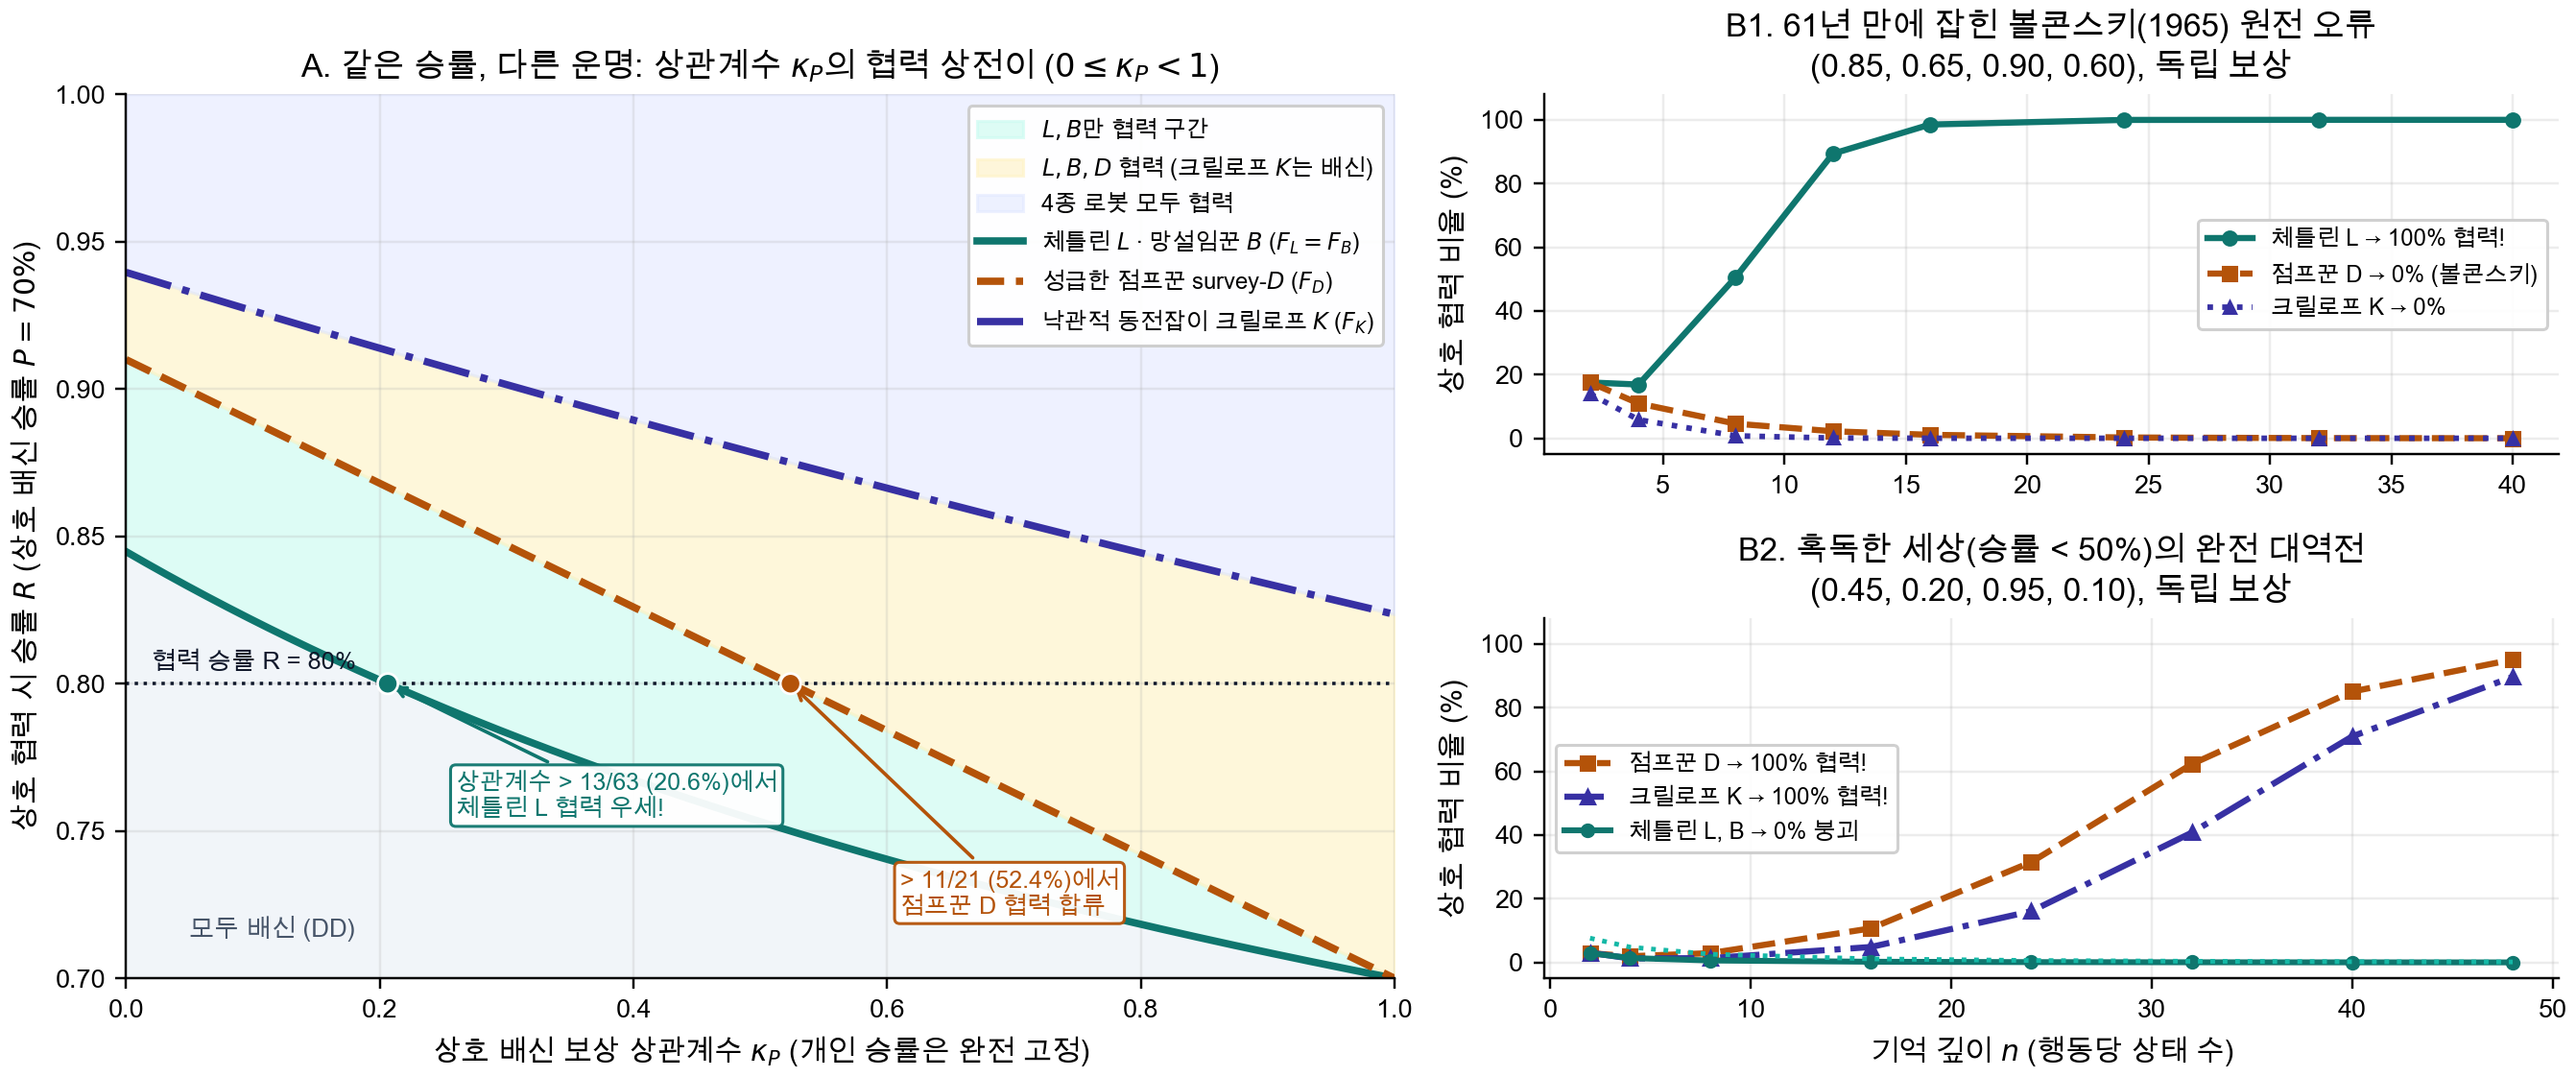
\includegraphics[width=0.94\textwidth]{figs/kr_fig1_shared_fate_and_volkonskii.png}
  \caption{\textbf{상관계수 $\kappa_P$의 협력 상전이, 61년 만의 볼콘스키 원전 오류, 그리고 혹독한 세상의 완전 역전.}
  (A) 개인 승률을 고정한 채 상관계수 $\kappa_P$만 높이면 $F_L=F_B < F_D < F_K$ ($0 \le \kappa_P < 1$) 순서로 협력 구간이 열린다.
  (B1) 볼콘스키(1965, p.~47) 원전 예제에서 점프꾼 $D$는 0\%로, 체틀린 $L$은 100\%로 갈라진다.
  (B2) $R<50\%, T+S>1$(대칭 상태 완전 지지, $0 \le \kappa_P < 1$)이고 $R>F_K>F_D$인 혹독한 세상에서는 반대로 $D, K$가 100\% 협력하고 $L, B$가 0\%로 무너진다.}
  \label{fig:kr1}
\end{figure}

\section{역설 2: 67\% 불완전 동기화의 기적과 기억 `+1칸'의 배신}

이제 두 로봇의 기억 길이가 다를 때를 보자. 앨리스는 밥보다 3배 더 끈질긴 기억을 갖고 있다($240$칸 vs $80$칸, 비율 $\gamma = 3$). 보수표는 $(0.80, 0.60, 0.90, 0.20)$이다. 직관대로라면 불운이 100\% 똑같이 찾아올수록 둘이 잘 맞을 것 같다. 결과는 정반대다:

\begin{wowbox}{보수 숫자와 무관한 황금 동기화 법칙 $\kappa_*(\gamma) = \dfrac{1+1/\gamma}{2}$}
\begin{itemize}
  \item \textbf{불운 동기화 0\% (완전 독립)}: 상호 협력률 \textbf{$9.08 \times 10^{-11}$} (완전 붕괴).
  \item \textbf{불운 동기화 100\% (완전 일치)}: 상호 협력률 \textbf{$2.15 \times 10^{-42}$} (더 처참한 붕괴!).
  \item \textbf{최적 상관계수 66.7\% ($\kappa_* = 2/3$) 주변}: 탈출 비용이 유일하게 최소화되며 협력률 \textbf{99.8529\%} ($B$는 \textbf{99.8943\%}) 대폭발!
\end{itemize}
\textbf{왜 그럴까?} 둘이 동시에 출구 문에 닿으려면 앨리스는 밥보다 순손실을 정확히 3배 더 겪어야 한다. 100\% 똑같이 패배하면 밥이 출구 문에 닿을 때 앨리스는 아직 160칸 깊은 곳에 남아 있어, 밥만 혼자 먼저 협력했다가 배신당하고 되돌아온다. 정확히 $\kappa_* = \frac{1+1/\gamma}{2}$일 때 앨리스가 단독 불운을 딱 필요한 비율로 맞아 탈출 비용이 유일하게 최소화되며, 두 카운터가 $3:1$ 대각선을 타고 출구 문에 도달한다!
\end{wowbox}

여기에 망설임꾼 $B$가 던지는 반전이 하나 더 있다. 동기화가 99\%로 너무 높을 때, 성실한 $L$은 짧은 기억의 밥이 문에 닿자마자 곧장 혼자 튀어나가 배신당한다. 반면 문 앞에서 동전을 던져 절반은 버티는 \textbf{망설임꾼 $B$}는 출구 문 바로 앞칸에서 앨리스가 따라올 때까지 기다려 준다! 그 결과 $(60,20)$ 기억 평면($R=0.80$)에서 성공 탈출 경로가 경계점 $(40,19)$를 방문할 확률이 $L$의 \textbf{0.63\%}에서 $B$의 \textbf{87.5\%}로 치솟고, 한 번의 탈출 시도 성공률이 무려 \textbf{8,994배} 폭증한다(그림~\ref{fig:kr2}B). 나아가 $(R=0.78, \gamma=2, \kappa_P=0.99)$ 게임에서는 이 경계 대기 효과가 실제 상전이까지 갈라놓아, \textbf{$L$의 상호 협력률은 0\%로, $B$의 상호 협력률은 100\%로 수렴한다!}

\begin{shockbox}{기억 `+1칸'의 배신: 나만 한 칸 더 똑똑해지면 사회가 붕괴한다}
100\% 동시 충격이 주어지는 죄수의 딜레마 $(0.55, 0.40, 0.99, 0.39)$에서, 두 로봇이 똑같이 행동당 40칸의 기억을 가지면 상호 협력률은 \textbf{99.9837\%}다. 그런데 로봇~1이 혼자 몰래 기억을 \textbf{딱 한 칸 늘려 41칸}으로 바꾸면 어떻게 될까?
\begin{itemize}
  \item 로봇~1의 개인 승률: \textbf{55.0\% $\longrightarrow$ 67.0\%} (큰 이득!)
  \item 사회 전체의 상호 협력률: \textbf{99.9837\% $\longrightarrow$ 0.0018\%} (완전 파괴!)
\end{itemize}
똑같은 40칸일 때는 동시 불운이 둘을 함께 출구 밖으로 밀어냈지만, 딱 1칸의 우위가 생기는 순간 41칸짜리가 배신에 한 걸음 더 남아 40칸짜리를 반복적으로 착취해 버린다(그림~\ref{fig:kr2}C). 심지어 $N \ge 3$명 공공재 게임에서도 단 한 명만 기억을 키우면 임계선 $d_* = h\frac{N-2}{N-1}$을 넘는 순간 나머지 $N-1$명 전원이 100\% 협력에서 \textbf{전원 배신}으로 추락한다!
\end{shockbox}

\begin{figure}[t]
  \centering
  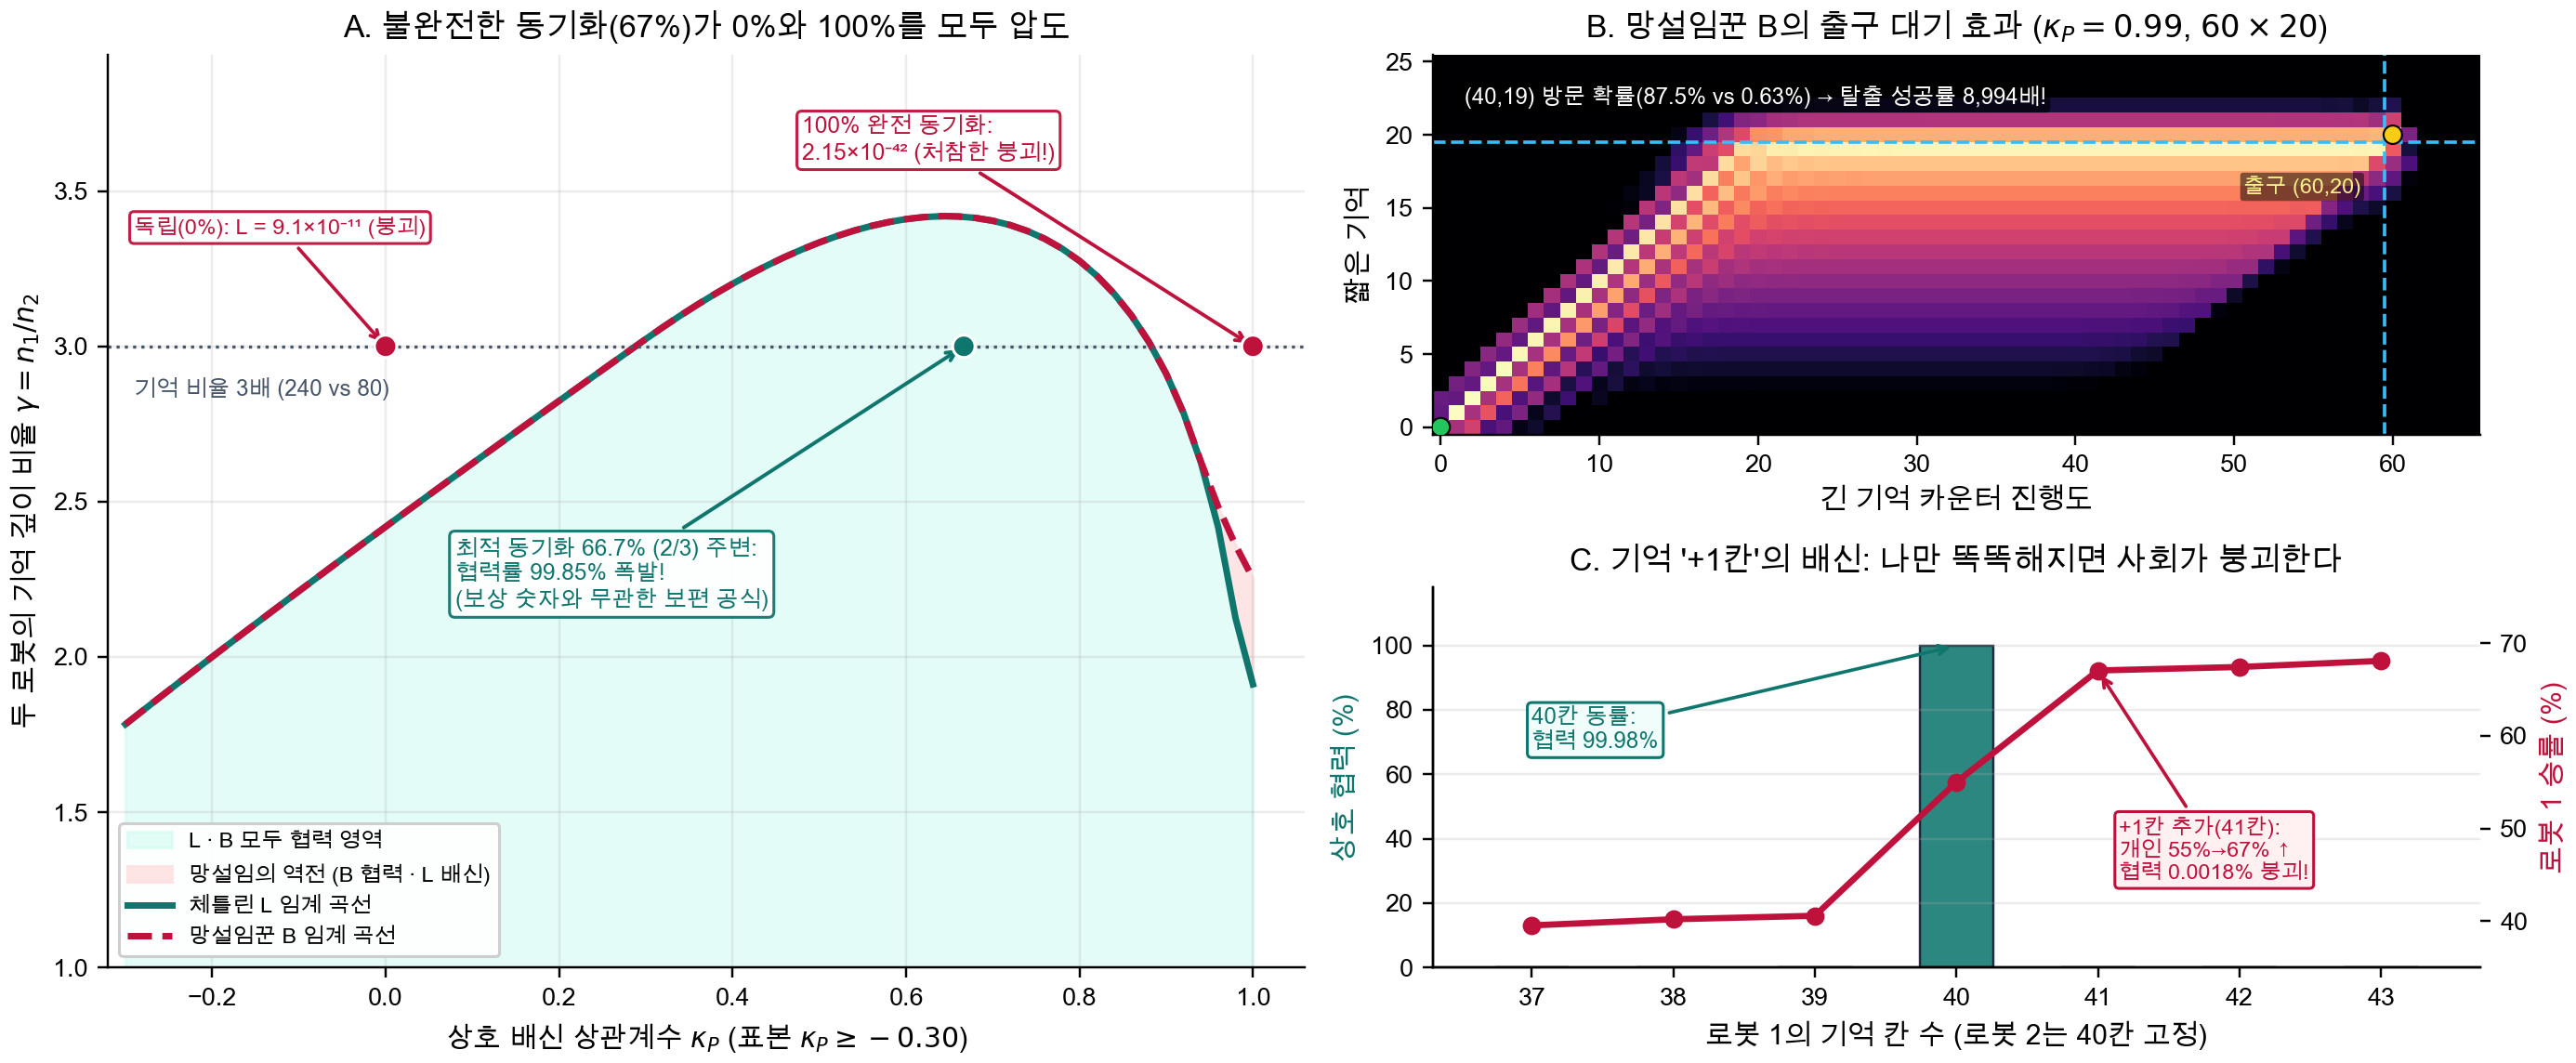
\includegraphics[width=0.94\textwidth]{figs/kr_fig2_imperfect_sync_and_plus1_cliff.png}
  \caption{\textbf{67\% 불완전 동기화의 기적, 망설임꾼 B의 8,994배 대기 효과, 그리고 `+1칸'의 배신.}
  (A) 기억 비율 3배(240 vs 80)에서는 0\%와 100\% 동기화 모두 붕괴하고, 최적 상관계수 $2/3$ 주변에서 99.85\% 협력이 솟아오른다.
  (B) $\kappa_P=0.99$에서 망설임꾼 $B$가 출구 문 앞 경계선을 따라 대기하는 밝은 능선(탈출 확률 8,994배).
  (C) $(40,40) \to (41,40)$으로 행동당 1칸만 늘려도 개인 승률은 67\%로 오르고 상호 협력은 0.0018\%로 추락한다.}
  \label{fig:kr2}
\end{figure}

\section{역설 3과 4: 사슴 사냥의 기억 신기루 \& 공정 동전의 3중 극한 상쇄}

\subsection{적당히 멍청해야 사슴을 잡는다 (열린 영역의 기억 신기루)}
두 사냥꾼이 안전하게 토끼를 잡으면 승률 80\%($P=T=0.80$), 둘이 힘을 합쳐 사슴을 잡으면 93--94\%($R$), 혼자 사슴을 쫓으면 약 50\%($S$)의 승률을 얻는다. 기억이 1칸뿐인 로봇들은 사슴 사냥에 37.5\%도 채 못 미친다. 그런데 기억을 12--30칸으로 키워주면 상호 사슴 사냥 비율이 \textbf{76--83\%로 치솟는다} --- 그리고 기억을 계속 더 키워주면 결국 \textbf{0\%로 완전히 무너져 버린다}!

놀라운 점은 이 `기억 신기루'가 $S=50\%$라는 면도날 경계 위의 우연이 아니라는 것이다. 우리는 단조 결합 증명과 정확 유리수 계산으로 $S=47\%\text{--}50\%$ 아래쪽 열린 영역과, $S=50\%$ 위쪽의 두 열린 영역($52\%$대 및 $55\%$대) 전체에서 `1칸 $< 37.5\%$, 중간 기억 $> 80\%$, 무한 기억 $\to 0\%$' 신기루가 발생하며, $S=50\%$ 양쪽에서 임계선 아래쪽($R < R_c(P, S)$)을 유지하며 결합 임계점 $(S, R) = (1/2, R_c(P, 1/2))$으로 다가가는 접근 경로들이 존재해, 어느 쪽에서 접근하든 적당한 기억의 정점이 \textbf{100\%에 한없이 가까워진 뒤 결국 0\%로 추락}함을 증명했다(그림~\ref{fig:kr3}A). 이유는 단순하다. 혼자 사슴을 쫓는 승률이 50\% 근처일 때, 카운터가 곧바로 포기하지 않고 기억 공간 안에서 앞뒤로 서성거리며 파트너가 합류할 `기회의 창'을 키워주기 때문이다($S=50\%$에서는 정확히 기억 깊이 $n$에 비례). 중간 깊이에서는 이 보너스가 승리하지만, 기억이 아주 커지면 미세한 지수적 불리함이 이를 압도해 끝내 0\%로 끌고 내려간다.

\subsection{공정 동전 경계(\texorpdfstring{$P=50\%$}{P=50\%})의 3중 극한 상쇄: \texorpdfstring{$3.43\text{배} \to 0.86\text{배} \to 1$}{3.43x -> 0.86x -> 1}}
상호 배신의 승률이 정확히 공정한 동전($P=50\%$, 독립 보상)일 때, 망설임꾼 $B$와 성실한 계단꾼 $L$이 배신의 늪에서 탈출하는 과정을 비교해 보자. 한 번의 탈출 시도 동안 기억 깊이 $N$이 커질수록:
\begin{enumerate}
  \item 두 로봇이 \textbf{동시에 출구 문에 도달}할 확률 비율($B/L$)은 $\frac{5(4-\pi)}{4\log 3 - \pi} \approx \mathbf{3.4258\text{배}}$로 수렴한다.
  \item 출구 문에 처음 도착해 \textbf{바로 다음 라운드에 즉시 동시 전환}할 확률 비율($B/L$)은 반대로 \textbf{0.8565배}로 낮아진다(도착 조건부로는 둘 다 동전을 던지므로 $1/4$배).
  \item 그런데 중간에 한 번도 배신당하지 않고 \textbf{배신에서 협력으로 깔끔하게 직행 탈출($DD \to CC$)}하는 최종 확률 비율($B/L$)은 정사각형($M=N=4096$)에서 $0.9995$($M=3N$에서는 $1.00025$)를 거쳐 극한에서 \textbf{정확히 1}로 수렴한다!
\end{enumerate}
왜 이런 마법 같은 상쇄가 일어날까? 망설임꾼 $B$는 문 앞에서 즉시 바뀌지 않고 머무르는 대신, 그 자리에서 빠져나가기 전에 문을 \textbf{여러 번 다시 두드릴 추가 기회}를 얻는다. 그 결과 `문 방문 비율 $\frac{4D_0}{D_{1/4}}$ $\times$ 즉시 전환 $\frac{1}{4}$ $\times$ 추가 노크 비율 $\frac{D_{1/4}}{D_0}$'가 극한에서 정확히 \textbf{1}로 상쇄되며(그림~\ref{fig:kr3}B), 정사각형($M=N$)에서는 두 로봇 모두 타원적분 상수 $\Gamma(1/4)^4/(128\pi)$가 지배하는 동일한 보편 법칙을 따른다!

\begin{figure}[t]
  \centering
  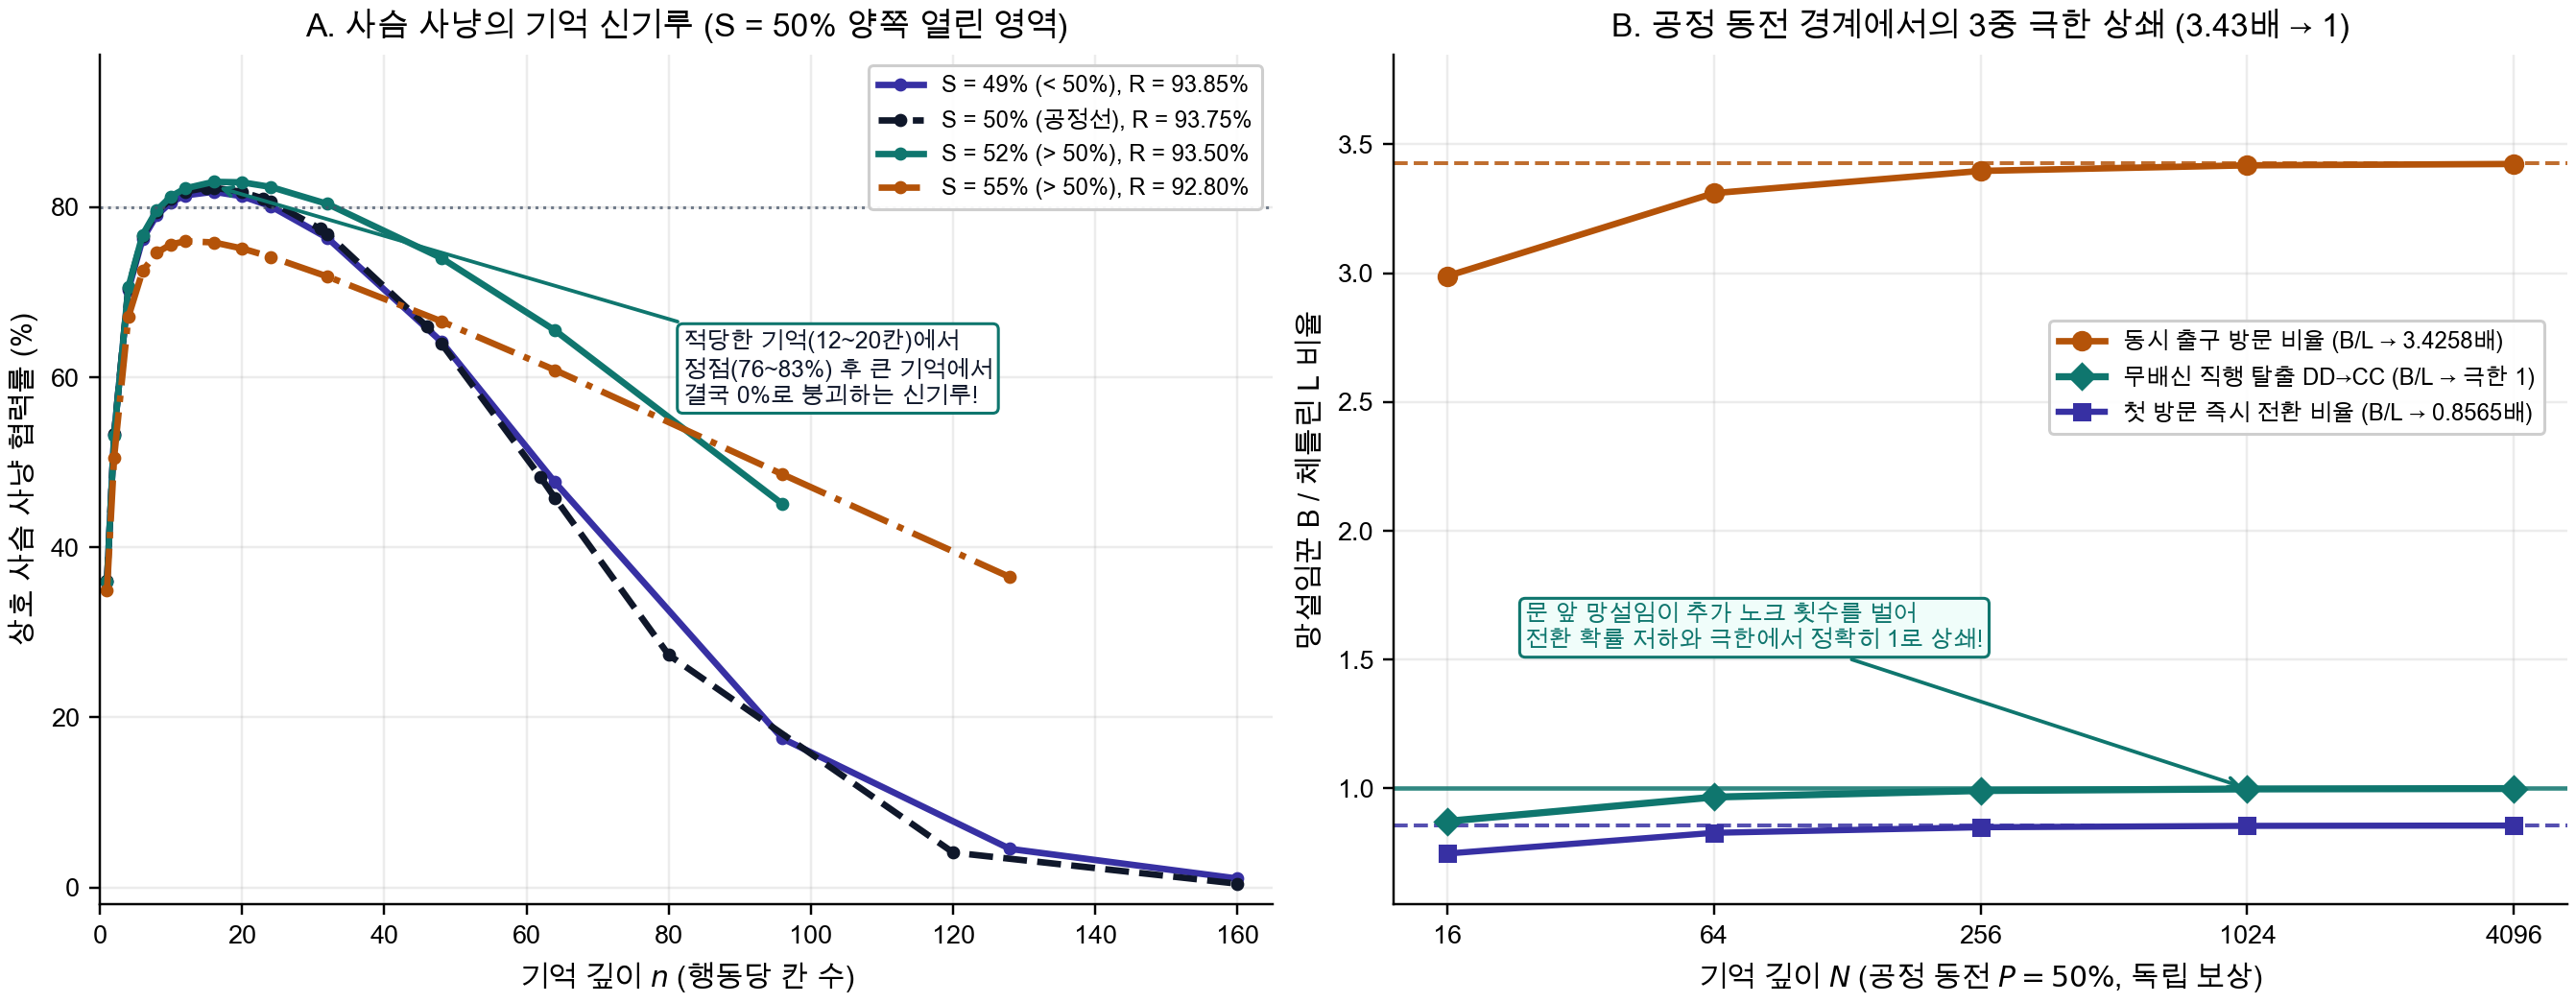
\includegraphics[width=0.94\textwidth]{figs/kr_fig3_staghunt_and_fair_cancellation.png}
  \caption{\textbf{사슴 사냥의 열린 영역 기억 신기루와 공정 동전 경계의 3중 극한 상쇄.}
  (A) $S=50\%$ 아래쪽(49\%)과 위쪽(52\%, 55\%) 모두에서 중간 기억에 협력이 급등(76--83\%)했다가 큰 기억에서 0\%로 붕괴한다.
  (B) $P=50\%$에서 망설임꾼 $B$와 체틀린 $L$의 비율: 동시 출구 방문은 3.4258배, 첫 방문 즉시 전환은 0.8565배로 갈리지만, 무배신 직행 탈출 비율은 $M=N=4096$에서 $0.9995$($M=3N$에서 $1.00025$)를 거쳐 극한에서 \textbf{정확히 1}로 수렴한다.}
  \label{fig:kr3}
\end{figure}

\section{역설 5: 60\% 골디락스 세금의 기적과 \texorpdfstring{$n_c = 2$}{n\_c = 2}의 즉각 붕괴}

1963년 겔판트·퍄테츠키-샤피로·체틀린이 집단 이기심을 해결하는 소련식 장치로 \textbf{공동 기금(\textit{Obshchaya kassa}, 완전 평균화)}을 도입했고, 1964년 긴즈부르크·크릴로프·체틀린이 이를 배치 게임에서 본격적으로 검증했다. 모든 시민의 보수를 100\% 한 통에 모아 똑같이 나누는 제도다. 우리는 이 아이디어를 확장해, 전체 보수 중 \textbf{일부 비율($\alpha$)만 공동 기금으로 모으는 부분 세금}을 대규모 마을($N \to \infty$) 공공재 게임에 적용해 보았다.

마을 주민 중 최소 \textbf{25\%}가 비용($0.60$)을 감수하고 봉사해야 마을 전체의 공공 사업이 성공해 기본 승률이 $0.80$에서 $0.97$로 오른다. 이론적으로 마을이 도달할 수 있는 최고 평균 후생은 딱 25\%만 봉사할 때의 \textbf{0.82}다.
\begin{itemize}
  \item \textbf{합리적이고 이기적인 인간(내시 균형)}: 봉사자 한 명이 정족수를 채워 얻는 이득보다 비용이 크므로, 세율이 \textbf{71.7\%($43/60$)} 미만인 한 대규모 마을에서 아무도 봉사하지 않는 것이 절대 유리하다.
  \item \textbf{기억 1칸짜리 눈먼 로봇($n=1$, $N \to \infty$ 극한)}:
    \begin{itemize}
      \item \textbf{0\% 세금 (완전 사유화)}: 사업 성공률 0\%, 사회 후생 \textbf{0.68}.
      \item \textbf{100\% 세금 (완전 공유)}: 보상이 모두 같아져 50\%가 맹목적으로 과잉 봉사한다. 낭비가 커져 사회 후생이 \textbf{0.67}로, 오히려 0\% 사유화보다 나빠진다!
      \item \textbf{60\% 부분 세금 (골디락스 기적)}: 합리적 인간이라면 전원 무임승차할 60\% 세율에서, 기억 1칸짜리 눈먼 시민들은 $N \to \infty$ 극한에서 저절로 \textbf{25\% 정족수}에 수렴해 사업 성공률 100\%, 이론적 최대 후생 \textbf{0.82}를 달성한다!
    \end{itemize}
\end{itemize}

\begin{shockbox}{기억이 1칸에서 2칸으로 늘어나면 기적은 즉사한다 ($n_c = 2$)}
그렇다면 이 눈먼 시민들에게 \textbf{기억을 딱 한 칸만 더($n=1 \to n=2$)} 주어 조금 더 똑똑하게 만들면 어떻게 될까? 놀랍게도 \textbf{합리적 인간을 이기는 기적이 그 즉시 완전히 사라진다!}
\begin{itemize}
  \item 정족수를 유지하는 최소 공유율이 60\%에서 \textbf{81.4\%($\frac{11-4\sqrt{3}}{5}$)}로 수직 상승해 내시 기준선(71.7\%)을 훌쩍 넘어버린다.
  \item 기억 2칸 이상($n \ge 2$)에서는 내시 기준선 이하의 어떤 세율($\alpha \le 71.7\%$)에서도 안정적인 공공재 공급점이 아예 존재하지 않으며, 마을 규모 $N$이 아무리 커져도 지워지지 않는 영구적 후생 손실이 남는다.
  \item 특히 세율 \textbf{70\%}, 기억 2칸에서는 평균장 역학에 국소적으로 끌리는 \textbf{3라운드 주기 호황-불황 궤도}가 존재해 세 번 중 딱 한 번만 공공재를 건설한다($L, B$ 모두 인증). 기억이 $n$칸으로 더 커지면 필요한 세율은 $100\% - 27.0\%/n$으로 치솟아, 결국 100\% 완전 공유가 아니면 정족수를 지킬 수 없게 된다(그림~\ref{fig:kr4}).
\end{itemize}
\textbf{왜 그럴까?} 기억 1칸일 때는 손실이 곧장 완만한 이탈로 이어져 인원을 25\%에 부드럽게 맞춘다. 하지만 기억이 2칸만 되어도 행동 전환이 가파른 S자 곡선으로 꺾이면서 고집과 과잉 반동이 생겨, 정족수 아래로 주저앉거나 3박자 출렁임에 빠지고 만다.
\end{shockbox}

\begin{figure}[t]
  \centering
  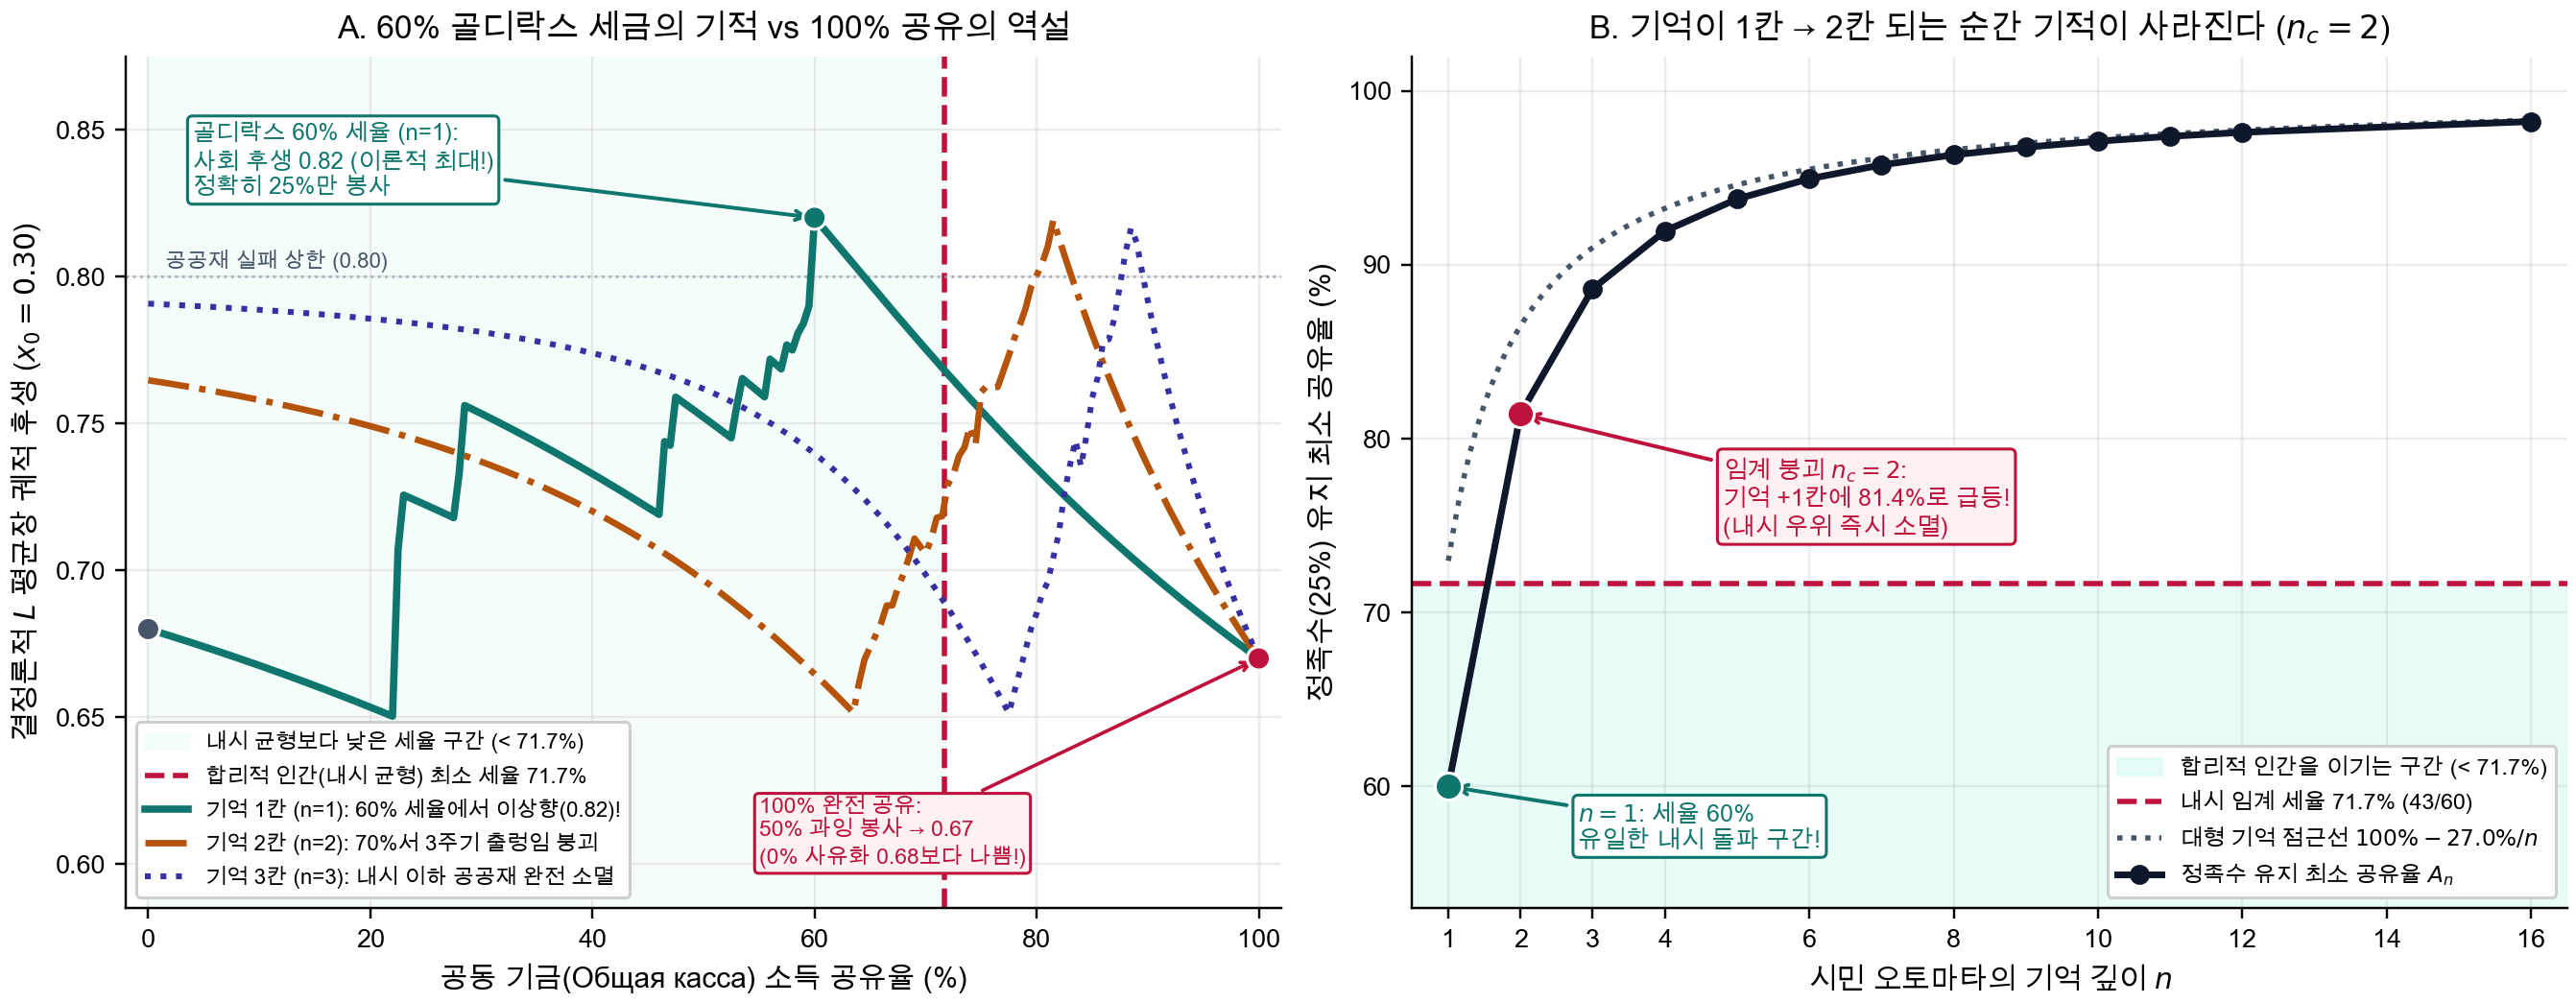
\includegraphics[width=0.94\textwidth]{figs/kr_fig4_goldilocks_tax_nc2.png}
  \caption{\textbf{60\% 골디락스 세금의 기적과 기억 2칸($n_c=2$)에서의 즉각 붕괴.}
  (A) 결정론적 $L$ 평균장 궤적 후생($x_0=0.30$, 800회 준비 반복 후 120회 평균)과 인증된 핵심 지점: 기억 1칸($n=1$) 시민은 내시 기준(71.7\%)보다 낮은 60\% 세율에서 이론적 최대 후생 0.82에 도달한다(0\%는 0.68, 100\%는 0.67).
  (B) 시민의 기억이 $n=1 \to 2$로 딱 1칸 늘어나는 순간 최소 공유율이 81.4\%로 뛰어오르며 내시 우위가 즉시 소멸하고, 깊은 기억에서는 $1/n$ 속도로 100\% 공유에 수렴한다.}
  \label{fig:kr4}
\end{figure}

\section{마무리: 핵심 대수 정리의 Lean 검증과 60년 만의 수학 고고학}

1960년대 모스크바의 잊힌 집단 오토마타 논문 10편을 원문 스캔(Math-Net.Ru)에서 직접 발굴해 현대의 대편차 이론, 타원적분, 대규모 평균장 역학으로 연결한 결과, 우리는 `단순함이 합리성을 이기고, 불완전한 동기화가 완벽한 동기화를 이기며, 기억 한 칸의 증가가 사회 전체를 무너뜨리는' 다섯 가지 정밀 법칙을 완성했다.

이 연구의 핵심 수치 결과는 데이터셋별 고정밀 연산과 정확 유리수 포아송 잔차 구간($n=80$ 충격 벤치마크 72자리, $(40,40)/(41,40)$ 잔차 폭 $4.0\times 10^{-70}$ 및 $1.76\times 10^{-66}$로 모두 $2\times 10^{-66}$ 미만, $(60,20)$ 탈출 격자 75자리 인증·150자리 작업 정밀도, $(240,80)$ 및 사슴 사냥 76자리 인증·최대 434자리 내부 정밀도, 공정 동전 스펙트럼 105자리 작업·82자리 출력, 3주기 궤도 $10^{-80}$ 수축 상자)으로 검증되었으며, 5개 핵심 정리의 대수적·마르코프 뼈대---\textbf{공개 정리 117개(보조 정리 포함 177개)}---는 외부 라이브러리 없는 독립형 \textbf{Lean~4.36.0} 증명 스위트(\texttt{sorry} 0개, 표준 공리만 사용, 전체 1,168개 선언 중 911개 정리 상수 공리 자동 감사 통과)로 완벽히 기계 검증되었다. 상세한 수학적 증명과 미해결 경계 문제는 두 편의 영문 학술 논문(Paper~1, Paper~2)에 수록되어 있다.

\end{document}
